\documentclass[a4paper,12pt,twoside]{memoir}

% Castellano
\usepackage[spanish,es-tabla]{babel}
\selectlanguage{spanish}
\usepackage[utf8]{inputenc}
\usepackage[T1]{fontenc}
\usepackage{lmodern} % scalable font
\usepackage{microtype}
\usepackage{placeins}
\usepackage{dirtree}
\usepackage{listings}


\RequirePackage{booktabs}
\RequirePackage[table]{xcolor}
\RequirePackage{xtab}
\RequirePackage{multirow}

\usepackage{tcolorbox}

% Links
\usepackage[colorlinks]{hyperref}
\hypersetup{
	allcolors = {red}
}

% Ecuaciones
\usepackage{amsmath}

% Rutas de fichero / paquete
\newcommand{\ruta}[1]{{\sffamily #1}}

% Párrafos
\nonzeroparskip


% Imagenes
\usepackage{graphicx}
\newcommand{\imagen}[2]{
	\begin{figure}[!h]
		\centering
		\includegraphics[width=0.9\textwidth]{#1}
		\caption{#2}\label{fig:#1}
	\end{figure}
	\FloatBarrier
}

\newcommand{\imagenflotante}[2]{
	\begin{figure}%[!h]
		\centering
		\includegraphics[width=0.9\textwidth]{#1}
		\caption{#2}\label{fig:#1}
	\end{figure}
}



% El comando \figura nos permite insertar figuras comodamente, y utilizando
% siempre el mismo formato. Los parametros son:
% 1 -> Porcentaje del ancho de página que ocupará la figura (de 0 a 1)
% 2 --> Fichero de la imagen
% 3 --> Texto a pie de imagen
% 4 --> Etiqueta (label) para referencias
% 5 --> Opciones que queramos pasarle al \includegraphics
% 6 --> Opciones de posicionamiento a pasarle a \begin{figure}
\newcommand{\figuraConPosicion}[6]{%
  \setlength{\anchoFloat}{#1\textwidth}%
  \addtolength{\anchoFloat}{-4\fboxsep}%
  \setlength{\anchoFigura}{\anchoFloat}%
  \begin{figure}[#6]
    \begin{center}%
      \Ovalbox{%
        \begin{minipage}{\anchoFloat}%
          \begin{center}%
            \includegraphics[width=\anchoFigura,#5]{#2}%
            \caption{#3}%
            \label{#4}%
          \end{center}%
        \end{minipage}
      }%
    \end{center}%
  \end{figure}%
}

%
% Comando para incluir imágenes en formato apaisado (sin marco).
\newcommand{\figuraApaisadaSinMarco}[5]{%
  \begin{figure}%
    \begin{center}%
    \includegraphics[angle=90,height=#1\textheight,#5]{#2}%
    \caption{#3}%
    \label{#4}%
    \end{center}%
  \end{figure}%
}
% Para las tablas
\newcommand{\otoprule}{\midrule [\heavyrulewidth]}
%
% Nuevo comando para tablas pequeñas (menos de una página).
\newcommand{\tablaSmall}[5]{%
 \begin{table}
  \begin{center}
   \rowcolors {2}{gray!35}{}
   \begin{tabular}{#2}
    \toprule
    #4
    \otoprule
    #5
    \bottomrule
   \end{tabular}
   \caption{#1}
   \label{tabla:#3}
  \end{center}
 \end{table}
}

%
%Para el float H de tablaSmallSinColores
\usepackage{float}

%
% Nuevo comando para tablas pequeñas (menos de una página).
\newcommand{\tablaSmallSinColores}[5]{%
 \begin{table}[H]
  \begin{center}
   \begin{tabular}{#2}
    \toprule
    #4
    \otoprule
    #5
    \bottomrule
   \end{tabular}
   \caption{#1}
   \label{tabla:#3}
  \end{center}
 \end{table}
}

\newcommand{\tablaApaisadaSmall}[5]{%
\begin{landscape}
  \begin{table}
   \begin{center}
    \rowcolors {2}{gray!35}{}
    \begin{tabular}{#2}
     \toprule
     #4
     \otoprule
     #5
     \bottomrule
    \end{tabular}
    \caption{#1}
    \label{tabla:#3}
   \end{center}
  \end{table}
\end{landscape}
}

%
% Nuevo comando para tablas grandes con cabecera y filas alternas coloreadas en gris.
\newcommand{\tabla}[6]{%
  \begin{center}
    \tablefirsthead{
      \toprule
      #5
      \otoprule
    }
    \tablehead{
      \multicolumn{#3}{l}{\small\sl continúa desde la página anterior}\\
      \toprule
      #5
      \otoprule
    }
    \tabletail{
      \hline
      \multicolumn{#3}{r}{\small\sl continúa en la página siguiente}\\
    }
    \tablelasttail{
      \hline
    }
    \bottomcaption{#1}
    \rowcolors {2}{gray!35}{}
    \begin{xtabular}{#2}
      #6
      \bottomrule
    \end{xtabular}
    \label{tabla:#4}
  \end{center}
}

%
% Nuevo comando para tablas grandes con cabecera.
\newcommand{\tablaSinColores}[6]{%
  \begin{center}
    \tablefirsthead{
      \toprule
      #5
      \otoprule
    }
    \tablehead{
      \multicolumn{#3}{l}{\small\sl continúa desde la página anterior}\\
      \toprule
      #5
      \otoprule
    }
    \tabletail{
      \hline
      \multicolumn{#3}{r}{\small\sl continúa en la página siguiente}\\
    }
    \tablelasttail{
      \hline
    }
    \bottomcaption{#1}
    \begin{xtabular}{#2}
      #6
      \bottomrule
    \end{xtabular}
    \label{tabla:#4}
  \end{center}
}

%
% Nuevo comando para tablas grandes sin cabecera.
\newcommand{\tablaSinCabecera}[5]{%
  \begin{center}
    \tablefirsthead{
      \toprule
    }
    \tablehead{
      \multicolumn{#3}{l}{\small\sl continúa desde la página anterior}\\
      \hline
    }
    \tabletail{
      \hline
      \multicolumn{#3}{r}{\small\sl continúa en la página siguiente}\\
    }
    \tablelasttail{
      \hline
    }
    \bottomcaption{#1}
  \begin{xtabular}{#2}
    #5
   \bottomrule
  \end{xtabular}
  \label{tabla:#4}
  \end{center}
}

%
% Nuevo comando para resaltar los términos en inglés.
\newcommand{\english}[1]{\emph{#1}}

%
% Nuevo comando para resaltar conceptos.
\newcommand{\concept}[1]{\textbf{#1}}

%
% Nuevo comando para resaltar nombres de archivo.
\newcommand{\filename}[1]{\texttt{#1}}

%
% Nuevo comando para URLs.
\newcommand{\myurl}[2]{\href{#1}{#2}\footnote{\url{#1}}}


\definecolor{cgoLight}{HTML}{EEEEEE}
\definecolor{cgoExtralight}{HTML}{FFFFFF}

%
% Nuevo comando para tablas grandes sin cabecera.
\newcommand{\tablaSinCabeceraConBandas}[5]{%
  \begin{center}
    \tablefirsthead{
      \toprule
    }
    \tablehead{
      \multicolumn{#3}{l}{\small\sl continúa desde la página anterior}\\
      \hline
    }
    \tabletail{
      \hline
      \multicolumn{#3}{r}{\small\sl continúa en la página siguiente}\\
    }
    \tablelasttail{
      \hline
    }
    \bottomcaption{#1}
    \rowcolors[]{1}{cgoExtralight}{cgoLight}

  \begin{xtabular}{#2}
    #5
   \bottomrule
  \end{xtabular}
  \label{tabla:#4}
  \end{center}
}




\graphicspath{ {./img/} }

% Capítulos
\chapterstyle{bianchi}
\newcommand{\capitulo}[2]{
	\setcounter{chapter}{#1}
	\setcounter{section}{0}
	\chapter*{#2}
	\addcontentsline{toc}{chapter}{#2}
	\markboth{#2}{#2}
}

% Apéndices
\renewcommand{\appendixname}{Apéndice}
\renewcommand*\cftappendixname{\appendixname}

\newcommand{\apendice}[1]{
	%\renewcommand{\thechapter}{A}
	\chapter{#1}
}

\renewcommand*\cftappendixname{\appendixname\ }

% Formato de portada
\makeatletter
\usepackage{xcolor}
\newcommand{\tutor}[1]{\def\@tutor{#1}}
\newcommand{\course}[1]{\def\@course{#1}}
\definecolor{cpardoBox}{HTML}{E6E6FF}
\def\maketitle{
  \null
  \thispagestyle{empty}
  % Cabecera ----------------
\noindent
\includegraphics[width=\textwidth]{cabecera}\vspace{1cm}%
  \vfill
  % Título proyecto y escudo informática ----------------
  \colorbox{cpardoBox}{%
    \begin{minipage}{.8\textwidth}
      \vspace{.5cm}\Large
      \begin{center}
      \textbf{TFG del Grado en Ingeniería Informática}\vspace{.6cm}\\
      \textbf{\LARGE\@title{}}
      \end{center}
      \vspace{.2cm}
    \end{minipage}

  }%
  \hfill\begin{minipage}{.20\textwidth}
    
\includegraphics[width=\textwidth]{escudoInfor}
  \end{minipage}
  \vfill
  % Datos de alumno, curso y tutores ------------------
  \begin{center}%
  {%
    \noindent\LARGE
    Presentado por \@author{}\\ 
    en Universidad de Burgos --- \@date{}\\
    Tutores: \@tutor{}\\
  }%
  \end{center}%
  \null
  \cleardoublepage
  }
\makeatother


% Datos de portada
\title{PDDetection\\ Aplicación de técnicas de minería de datos para la detección de la enfermedad del Parkinson \\Documentación Técnica}
\author{Adrián Arnaiz Rodríguez}
\tutor{Jose Francisco Díez Pastor y César Ignacio García Osorio}
\date{\today}

\begin{document}

\maketitle



\cleardoublepage



%%%%%%%%%%%%%%%%%%%%%%%%%%%%%%%%%%%%%%%%%%%%%%%%%%%%%%%%%%%%%%%%%%%%%%%%%%%%%%%%%%%%%%%%



\frontmatter


\clearpage

% Indices
\tableofcontents

\clearpage

\listoffigures

\clearpage

\listoftables

\clearpage

\mainmatter

\appendix

\apendice{Plan de Proyecto Software}

\section{Introducción}
En este apartado se desarrollará la planificación temporal del proyecto, así como también un estudio de viabilidad.

\section{Planificación temporal}
Para la planificación temporal del proyecto, se sigue una metodología \english{Scrum}. Se realizarán diferentes \english{sprints}, en los que se marcaban objetivos. Idealmente, los \english{sprints} duran dos semanas. Debido a carga de trabajo externa a este proyecto, esta duración se ha visto afectada y se han realizado \english{sprints} de más y menos duración. Durante cada uno de ellos, se irán creando y realizando las diferentes tareas correspondientes a los objetivos fijados en cada \english{sprints}. Al finalizar cada \english{sprint}, se realizan reuniones con los tutores para revisar los objetivos cumplidos y marcar unos nuevos. 

Se ha utilizado Github para el seguimiento de la aplicación, ayudados por el tablero Kanban de Zen-hub. Esta herramienta nos ha permitido llevar un seguimiento más detallado de la planificación en cada momento. El repositorio del proyecto, y las issues realizadas se encuentra en el \myurl{https://github.com/AdrianArnaiz/TFG-Neurodegenerative-Disease-Detection}{repositorio del proyecto}.

A su vez, cabe destacar que los primeros \english{sprints} no se muestran de manera correcta. Esto es debido al fallo de no cerrar los \english{sprints} en github, por lo que los gráficos \english{Burndown} están alterados.

\subsection{Sprint 1}
Idealmente, el comienzo de este sprint comenzaba el 15 de Diciembre. Debido a cargas de trabajo externas al proyecto, al final se comenzó el 14 de febrero. Duración del sprint: 14 de febrero 2019 al 28 de febrero 2019. Ver gráfico \english{Burndown} en la figura \ref{fig:sprint1}.
\imagen{sprint1}{Burndown chart del sprint 1}
Tareas realizadas:
\begin{itemize}
\item Instalación del cliente Github: GitTortoise.
\item Crear la estructura de directorios del repositorio.
\item Instalación de \LaTeX{} y todos sus componentes. 
\item Lectura en profundidad de dos artículos de Giovanni Dimauro: \cite{giovanni1} y \cite{giovanni2} . 
\end{itemize}
En este sprint se realizó la fase inicial del proyecto, que comprendía desde la instalación y creación de elementos principales, hasta la iniciación de la investigación.


\subsection{Sprint 2}
Duración del sprint: 28 de febrero de 2019 al 13 de marzo de 2019. Ver gráfico \english{Burndown} en la figura \ref{fig:sprint2}.
\imagen{sprint2}{Burndown chart del sprint 2}
Tareas realizadas:
\begin{itemize}
\item Realizar la taxonomía de las características extraídas de cada audio, qué características de cada tipo...
\item Identificar las herramientas de extracción de características de audio.
\item Realizar taxonomía de correspondencia entre las herramientas y las características concretas a extraer.
\item Realizar un arreglo en la preservación de privacidad de los audios del conjunto de datos. Los audios son audios privados definidos en \cite{OrzCorpus}. Por un error con los archivos ignorados por \textit{Git}, se subieron algunos audios. Se tuvieron que borrar para mantener la privacidad de los mismos.
\end{itemize}
En este sprint, seguimos explorando el estado del arte ahora de manera más precisa: empezar a ver en profundidad el proceso de extracción de características y medidas de los audios, explorando en diferentes artículos que características extraer y buscando las herramientas necesarias para su extracción.

\subsection{Sprint 3}
Duración del sprint: 13 de marzo 2019 al 29 de marzo 2019. Ver gráfico \english{Burndown} en la figura \ref{fig:sprint3}.
\imagen{sprint3}{Burndown chart del sprint 3}
Tareas realizadas:
\begin{itemize}
\item Búsqueda de audios, peticiones y realización de taxonomía de audios encontrados.
\item Lectura en profundidad de los artículos más importantes del estado del arte, i.e. \cite{Orz2016}.
\item Finalización de exploración del estado del arte: realizar taxonomía y resúmenes.
\end{itemize}
En este sprint se llevó a cabo la finalización de estado del arte y su resumen de aspectos y artículos más importantes. Un aspecto importante fue la búsqueda de audios, trabajo bastante arduo dentro del proyecto debido a que son muy difíciles de encontrar. Empezamos el proceso de extracción de características descrito en \cite{Orz2016}: instalación y familiarización de librerías, segmentación de audios, etc...

\subsection{Sprint 4}
Duración del sprint: 29 de marzo 2019 al 11 de abril 2019. Ver gráfico \english{Burndown} en la figura \ref{fig:sprint4}.
\imagen{sprint4}{Burndown chart del sprint 4}
Tareas realizadas:
\begin{itemize}
\item Instalar herramientas de manejo de audio como Disvoice.
\item Explorar el funcionamiento de estas herramientas.
\item Preprocesar los audios: eliminar silencios inicial y final.
\item Extracción de diferentes características de los audios con Disvoice.
	\begin{itemize}
    \item Extracción medidas prosódicas de audios completos.
	\item Extraer medidas de fonación de \english{voiced frames} de vocales y frase.
	\item Extraer medidas de articulación (cepstrales y de energía de transiciones).
	\end{itemize}
\end{itemize}
Se realizó el proceso de extracción de características. Se recorre toda la estructura de audios para crear las correspondientes matrices de características (en numpy) de cada tipo de audio y así dejar preparados los datos para entrenar modelos. Hay una matriz de características por cada tipo de audio y cada tipo de características. Para ello se realizó desde la instalación y comprensión del funcionamiento de las herramientas de manejo de audio, hasta extraer las medidas completas con la herramienta Disvoice.

\subsection{Sprint 5}
Duración del sprint: 15 de abril 2019 al 2 de mayo 2019. Ver gráfico \english{Burndown} en la figura \ref{fig:sprint5}.
\imagen{sprint5}{Burndown chart del sprint 5}
Tareas realizadas:
\begin{itemize}
\item Documentación de avances hasta el momento.
\item Realización de los \textbf{primeros experimentos} con clasificadores, incluyendo la limpieza de características necesaria para ello. Se realiza, como mínimo, el proceso de \cite{Orz2016}. Se utilizan las características extraídas con \textit{Disvoice}.
\item Realización proyección de características.
\item Investigación, documentación y aprendizaje sobre \english{Deep Learning}.
\end{itemize}
En este sprint, se documentó el trabajo realizado hasta el momento. También se realizó el estudio con clasificadores para los conjuntos de características extraídos con Disvoice. Probamos proyecciones de datos de estas características para graficarlos. En este sprint se comenzó la investigación y aprendizaje sobre Deep Learning, para su aplicación a posteriores sprints.


\subsection{Sprint 6}
Duración del sprint: 2 de mayo 2019 al 17 de mayo 2019. Ver gráfico \english{Burndown} en la figura \ref{fig:sprint6}.
\imagen{sprint6}{Burndown chart del sprint 6}
Tareas realizadas:
\begin{itemize}
\item Búsqueda de librerías de \english{Deep Learning} para audios.
\item Modificación de las características Disvoice.
\item División del conjunto de datos por sexo.
\item Realización de \textbf{segundos experimentos} con características Disvoice modificadas. Se describe la segunda fase en la memoria en el apartado Aspectos Relevantes. Se realiza, como mínimo, el proceso de \cite{Orz2016}, pero añadiendo edad y sexo a las características extraídas y dividiendo los conjuntos por sexo.
\end{itemize}
En este \textit{sprint} realizamos la modificación de las características de \textit{Disvoice} (adición de edad y sexo, división por sexos...) y realizamos los experimentos con estas nuevas características. También, siguiendo la línea del anterior \textit{sprint}, profundizamos más en el \english{Deep Learning}, Buscando bibliotecas para la extracción de características de nuestros audios.

\subsection{Sprint 7}
Duración del sprint: 17 de mayo 2019 a 14 de junio 2019. Ver gráfico \english{Burndown} en la figura \ref{fig:sprint7}.
\imagen{sprint7}{Burndown chart del sprint 7}
Tareas realizadas:
\begin{itemize}
\item Arreglo de fallo encontrado.
\item Repetición de primeros y segundos experimentos: incluye repetición de análisis y resumen de resultados.
\item Instalación biblioteca VGGish (y VGGish2Keras).
\item Realizar extracción de características con VGGish (VGGish2Keras).
\item Realización \textbf{terceros experimentos} con características VGGish. Se hace los experimentos con los embeddings y espectros extraídos con \textit{VGGish} \cite{vggish} .
\item Análisis de viabilidad comercial: \english{lean canvas}.
\end{itemize}
En la reunión previa a este sprint, se revisó el código y encontramos un fallo de \concept{data snooping}. No hacíamos validación cruzada anidada (\english{nested CV}). Debido a esto, tuvimos que arreglar el error y repetir los experimentos realizados hasta el momento (primeros y segundos con características Disvoice). Tras finalizar, tuvimos que volver a analizar y resumir todos los resultados de los experimentos, aunque estos habían variado menos de lo esperado. También, siguiendo con la línea de anteriores \textit{sprints}, realizamos la instalación de la biblioteca \textit{VGGish} de \english{Deep Learning}, extrajimos las características de los audios con esta biblioteca y realizamos los experimentos con estas nuevas características. Para finalizar, y por pedido de la OTRI (Oficina de transmisión de información de la Universidad de Burgos), se realizó un análisis de viabilidad comercial, concretamente un \english{lean canvas} de nuestro proyecto.

Cabe destacar que la duración de este \textit{sprint} es bastante mayor de lo normal. Se debe a dos aspectos. El primero de ellos es que la carga de trabajo de este \textit{sprint} era sustancialmente superior a los demás. Se debe a que en fallo encontrado requería de una repetición de gran parte del trabajo y además no podíamos frenarnos en los experimentos con \english{Deep Learning}. Por otra parte, coincidió con las dos últimas semanas del curso, las cuales estaban repletas de trabajos finales y exámenes de convocatoria, que hacían que el tiempo dedicado al proyecto tuviera que ser menor.

\subsection{Sprint 8}
Duración del sprint: 14 de junio 2019 a 24 de junio 2019. Ver gráfico \english{Burndown} en la figura \ref{fig:sprint8}.
\imagen{sprint8}{Burndown chart del sprint 8}
Tareas realizadas:
\begin{itemize}
\item Aprendizaje del patrón de diseño mediador-fachada.
\item Realización de la aplicación de escritorio.
\end{itemize}
En este sprint se realizó la aplicación demostrativa de escritorio. Para ello, se sugirió hacer mediante el patrón de diseño mediador-fachada. Por ello antes de realizar la aplicación se tuvo que comprender ese patrón. Una vez comprendido se realizó la aplicación. Como ya hemos comentado en la memoria principal, esta aplicación, aunque es la parte más vistosa, personalmente no la considero la parte más importante del proyecto. Únicamente es una aplicación que muestra una posible aplicación del resultado de este investigación, y que con las líneas de investigación futuras pudiera llegar a un producto funcional y estable.

\subsection{Sprint 9}
Duración del sprint: 24 de junio 2019 a 1 de junio 2019. Ver gráfico \english{Burndown} en la figura \ref{fig:sprint1}.
\imagen{sprint9}{Burndown chart del sprint 9}
Tareas realizadas:
\begin{itemize}
\item Revisión de la memoria hasta el momento.
\item Finalización de la memoria.
\item Búsqueda de documentación de pruebas unitarias en Minería de Datos.
\item Realización documentación de las clases.
\item Realización test unitarios.
\item Finalización de los anexos y el anexo de investigación donde detallamos las taxonomías.
\end{itemize}
En este último sprint se hicieron las últimas tareas del proyecto. Se terminó toda la documentación, lo que comprendía desde revisar lo hecho anteriormente, realizar lo que faltaba por terminar y buscar información sobre pruebas unitarias en el campo de la minería de datos.

\subsection{Frecuencia de código}
Añadimos la gráfica de frecuencia de código, donde se ve como se han distribuido las adiciones y modificaciones de código a lo largo del proyecto. Ver Figura \ref{fig:codefrequency}

\imagen{codefrequency}{Frecuencia de código}

\section{Estudio de viabilidad}
En este apartado se abordará la viabilidad económica, comercial y legal de este proyecto.

\subsection{Viabilidad económica}
En este apartado, simularemos el coste del proyecto que tendría en una empresa, o en una venta al público.
\subsubsection{Coste personal}
Este proyecto cuenta con dos \textbf{profesores contratados} durante 6 meses para este proyecto. Por cada profesor se asignan 0,5 créditos, por lo que el coste\footnote{\url{https://www.ubu.es/sites/default/files/portal_page/files/pdi_laboral_2019.pdf}} por tutor consideramos que es el siguiente:
\begin{itemize}
\item Sueldo ayudante doctor: 26445,24 euros anuales. Más 2 trienios más el complemento de mejora: $26445,24 + 1260,58 + 1110,71 = 28816,52$. En total imparte 24 créditos por lo que el coste anual por crédito es de 1200,68 euros. El coste total es el siguiente:
\begin{equation}
1200,68 \cdot 0,5 créditos = 600,34 euros
\end{equation}
\item Sueldo medio anual de un titular: 42220,34 euros anuales. En total imparte 24 créditos por lo que el coste anual por crédito es de 1759,18 euros. El coste total es el siguiente:
\begin{equation}
1759,18 \cdot 0,5 créditos = 879,59 euros
\end{equation}
\end{itemize}

También cuanta con un desarrollador del proyecto. Supondremos un salario bruto de 2000 euros para el desarrollador. Habrá que tener en cuenta los \myurl{http://www.seg-social.es/wps/portal/wss/internet/Trabajadores/CotizacionRecaudacionTrabajadores/}{gastos de seguridad social}. 
\begin{itemize}
\item Cotización por parte de la empresa: 23.6\%
\item Cotización por parte del empleado: 4.7\%
\item \textbf{Total: 28.3\%}
\end{itemize}
Por lo tanto el coste del desarrollador se detalla en \ref{tabla:costespersonales}
\tablaSmallSinColores{Costes de personal}{p{6.4cm} p{2.15cm} p{8cm}}{costespersonales}{
  \multicolumn{1}{p{4.5cm}}{\textbf{Concepto}} & \textbf{Coste{}}\\
 }
 {
  Salario mensual neto  & \multicolumn{1}{r}{1217.25}\\
  Retención IRPF (15\%) & \multicolumn{1}{r}{216.75}\\
  Seguridad social  (28.3\%) & \multicolumn{1}{r}{566}\\
  Salario mensual bruto  & \multicolumn{1}{r}{2000}\\\hline
  \textbf{Coste total (6 meses)}  & \multicolumn{1}{r}{12000}\\\hline
  }


\subsubsection{Coste informático}

El coste informático es mínimo. Se ha utilizado un único portátil personal. Su coste fue de 800 euros y se supone una amortización de 5 años. Para ello se contabilizará únicamente el cose amortizado. 
\begin{equation}
(800 / (12 \cdot 5)) \cdot 6 = 80 euros
\end{equation}

\subsubsection{Ingresos}
Para este proyecto se ha contado con la concesión de la beca prototipos de la Oficina de Transmisión de Información de la Universidad de Burgos. La cuantía de la beca ha sido de 800 euros, por lo que estos serán los ingresos del proyecto.

\subsubsection{Coste Total}
El coste total se detalla en la tabla \ref{tabla:costetotal}

\tablaSmallSinColores{Coste Total}{p{6.4cm} p{2.15cm} p{8cm}}{costetotal}{
  \multicolumn{1}{p{4.5cm}}{\textbf{Concepto}} & \textbf{Coste{}}\\
 }
 {
  Coste desarrollador  & \multicolumn{1}{r}{12000}\\
  Costes Tutores(15\%) & \multicolumn{1}{r}{1479.93}\\
  Hardware & \multicolumn{1}{r}{80}\\\hline
  Beca prototipos  & \multicolumn{1}{r}{-800}\\\hline
  \textbf{Coste total (6 meses)}  & \multicolumn{1}{r}{12679.93}\\\hline
  }



\subsection{Viabilidad comercial}
Para analizar la viabilidad comercial, realizaremos un \english{lean canvas}, \ref{fig:LeanCanvas}, la cual es una herramienta de análisis de negocio desarrollada por Alex Osterwalder \cite{osterwalder2007business}.

\begin{figure}[!h]
		\centering
		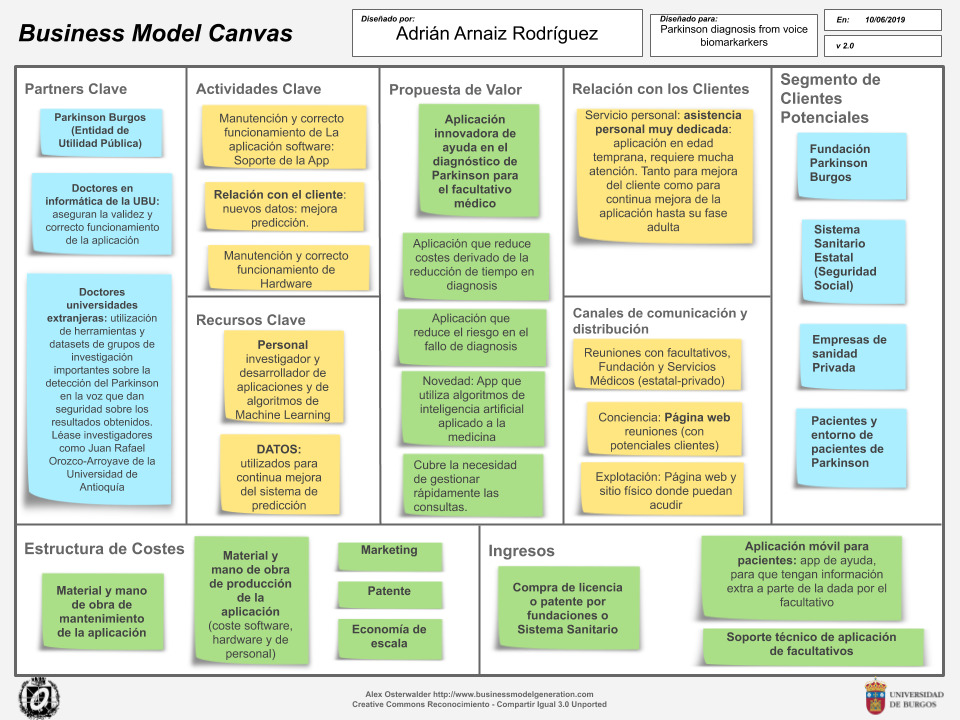
\includegraphics[width=1.1\textwidth]{LeanCanvas}
		\caption{Lean Canvas del proyecto}\label{fig:LeanCanvas}
\end{figure}


\subsection{Viabilidad legal}
Todo el código utilizado es de dominio público. Hemos utilizado multitud de librerías del lenguaje Python, las cuales son todas de dominio público. Las herramientas más concretas que hemos utilizado han sido las siguientes.
\begin{itemize}
\item \textbf{Disvoice}: alojado en \myurl{https://github.com/jcvasquezc/DisVoice}{repositorio público} de Github. \textbf{Tiene la licencia pública MIT}.
\item \textbf{VGGish}: alojado en \myurl{https://github.com/tensorflow/models/tree/master/research/audioset}{repositorio público de Github}.Pertenece al proyecto de Tensorflow. \textbf{Tiene la licencia pública Apache license 2.0}.
\end{itemize}
Todas las demás librerías utilizadas son propias de Python. También mencionar que no utilizamos el repositorio Disvoice original, sino que le hemos modificado para la ejecución en Windows. Esto ha sido posible ya que la licencia MIT permite tanto el uso comercial como la modificación el mismo.


\apendice{Especificación de Requisitos}

\section{Introducción}

\section{Objetivos generales}

\section{Catalogo de requisitos}

\section{Especificación de requisitos}



\apendice{Especificación de diseño}

\section{Introducción}
En éste apéndice, se describirán cómo están implementados los datos de esta aplicación, cuales son los procedimientos más relevantes de la aplicación, y cómo se organizan los proyectos en paquetes.

\section{Diseño de datos}
En este sección, explicaremos como están organizados tanto el conjunto de audios obtenido, cómo son y como se organizan las características extraídas de los audios, y el diagrama de clases de la aplicación.

\subsection{Conjunto de audios}
El conjunto de audios es el descrito en \cite{OrzCorpus}. También lo hemos descrito en la sección 5.3 de la memoria principal. Estos audios no se encuentran en el repositorio, ya que son de carácter privado. En \cite{OrzCorpus} se describe como: ``(...)incluye grabaciones de voz de 50 personas con PD y 50 controles sanos, 25 hombres y 25 mujeres en cada grupo. Todos los participantes son hablantes nativos de español colombiano. La edad de los hombres con PD varía de 33 a 77 años (media 62.2 $\pm$ 11.2), la edad de las mujeres con PD varía de 44 a 75 años (media 60.1 $\pm$ 7.8). Para el caso de los controles sanos, la edad de los hombres varía de 31 a 86 (media 61.2 $\pm$ 11.3) y la edad de las mujeres de 43 a 76 años (media 60.7 $\pm$ 7.7). Por lo tanto, la base de datos está bien equilibrada en términos de edad y género. Las grabaciones fueron capturadas en condiciones de control de ruido, en una cabina de prueba de sonido que se construyó en la Clínica Noel, en Medellín, Colombia. Los registros se muestrearon a 44100 Hz con 16 bits de resolución, utilizando un micrófono omnidireccional dinámico (Shure, SM 63L) que se usa comúnmente para aplicaciones profesionales. Las grabaciones se capturaron utilizando una tarjeta de audio profesional de hasta 24 bits y de tal forma que admite hasta 96 Kbps de frecuencia de muestreo (M-Audio, Fast Track C400). Estos audios están en formato wav." (p.343). Tendremos 100 audios de una frase y 100 audios de cada una de las 5 palabras. En caso de las vocales, tenemos 300 audios para cada vocal, en vez de 100, ya que hay 3 audios para cada vocal de cada persona. Aunque en el total hacen un número de audios de 2100 audios, como hemos comentado en la memoria, no se puede entrenar con todos a la vez. Tenemos que entrenar los modelos con las características extraídas de cada grupo de 100 o 300 audios (si son vocales) por separado. Esto hace que entrenemos los modelos con bases de datos pequeñas y corran riesgo de sobreajustarse.

Destacar también, que tenemos un archivo tipo excel donde se indica: edad,sexo, UPDRS, HY y tiempo desde la detección de la enfermedad del paciente. Este archivo se encuentra en \texttt{doc/masRecursos/PCGITA\_metadata.xlsx}.

\subsection{Características extraídas}
Como se ha comentado el la memoria hemos extraído diferentes características de los audios. Todas, se encuentran el el directorio o subdirectorios de \texttt{src/CaracterísticasExtraídas}. También, todas ellas están guardadas de manera serializada en formato tipo \english{numpy} con la herramienta \english{pickle}. Las características extraídas son las siguientes

\begin{itemize}
\item \textbf{Características Disvoice (primera fase):} se encuentran en \texttt{src/ CaracterísticasExtraídas} y se extraen en el \textit{notebook} \texttt{Extracción de características.ipynb} del directorio \texttt{src}. Están descritas más en detalle en la memoria en la sección 5.5.2 (Aspectos Relevantes - Primera Fase: atributos Disvoice - Modelado del discurso). A grandes rasgos, de los audios de la frase sacamos medidas de fonación, articulación y prosodia; de los audios de cada palabra sacamos medidas de fonación y articulación, y de los audios de cada vocal sacamos únicamente medidas de fonación. Hay un total de \textbf{18 conjuntos} diferentes de características. El tamaño de las matrices de características es el siguiente
	\begin{itemize}
	\item Fonación: 100$\times$30 y 300$\times$30 (para vocales). Se sacan 29 medidas más la clase. 
	\item Articulación: 100$\times$489. Se sacan 488 medidas más la clase.
	\item Prosodia: 100$\times$39. Se sacan 28 medidas más la clase.
	\end{itemize}

\item \textbf{Características MODIFICADAS Disvoice (segunda fase):} se encuentran en \texttt{src/ CaracterísticasExtraídas/EdadYSexo} y en \texttt{src/CaracterísticasExtraídas/DivisionSexo} y se extraen en \texttt{src/ Extracción de características MODIFICADAS Disvoice.ipynb}. Están descritas más en detalle en la memoria en la sección 5.6.1 (Aspectos Relevantes - Segunda Fase - Modelado del discurso). A grandes rasgos, primero se ha añadido los atributos edad y sexo a las anteriores características, por lo que tendremos otros 18 conjuntos de datos nuevos nuevos, cuya medida de las matrices es igual que la primera fase, pero teniendo 2 columnas más (2 características más). Por otro lado, se han dividido entre hombres y mujeres, por lo que tendremos otros 35 conjuntos de datos más, cada uno con la mitad de instancias que el original (tamaño: tendrán la mitad de filas que los de la fase 1, y tendrán 1 columna más: la edad). Por último, tenemos los conjuntos de características exactos a los de Orozco, solo los MFCC. Estos también están divididos por sexo. De estos últimos tenemos 24 conjuntos, cuyo tamaño es 50$\times$35 (34 medidas más la clase). Por lo hque forman un total de \textbf{78 conjuntos} de características diferentes.

\item \textbf{Características VGGish (tercera fase):} se encuentran en:
\begin{itemize}
\item \texttt{src/CaracterísticasExtraídas/vggish/embeddings}
\item \texttt{src/CaracterísticasExtraídas/vggish/espectros}.
\end{itemize}  
Están descritas más en detalle en la memoria en la sección 5.7.1 (Aspectos Relevantes - Tercera Fase - Modelado del discurso), y en los \textit{notebooks}. Se extraen para los tipos de audio de las 5 vocales y la frase los \textit{embeddings}, que genera unas matrices de características de tamaño 100$\times$256 para la frase y 300$\times$256 para cada vocal. Esto es debido a que \textit{VGGish} nos saca 128 \textit{embeddings} para cada fragmento de 25ms de un audio, y nosotros, hemos decidido que para formar un único array de cada audio, hacer la media y desviación de los \textit{embeddings}. Por otro lado, sacamos también los espectros de frecuencia del audio, con la herramienta del pre-procesado de VGGish. Los detalles se encuentran en la memoria, en el apartado recientemente indicado. El tamaño de las matrices de datos de los espectros es de 100$\times$128 para la frase y 300$\times$128 para cada vocal. Al igual que antes, es debido a que VGGish nos da 64 espectros de cada fragmento de 25ms, y hemos hecho la media y la desviación para tener un único array.
	
\end{itemize} 

\subsection{Diagrama de clases de la aplicación}
En este apartado se comentara las clases realizadas por nosotros en el proyecto. Es decir, las clases que se han creado para ayudar a los experimentos y realizar la aplicación. Señalamos que, únicamente se analizaran las realizadas por nosotros, todas la estructura de \textit{VGGish} no será analizada. De echo, por ejemplo, \textit{VGGish2Keras} es un conjunto de módulos con funciones, que no contienen ninguna clase.

\subsubsection{Clases de la etapa de experimentación}
 Cabe destacar que, en los experimentos con los clasificadores, se ha utilizado los \textit{notebooks} de \textit{Jupyter} para su realización. Por ello, en la etapa de realización de experimentos únicamente se realizaron 3 clases, sin ninguna relación entre ellas, las cuales únicamente se usaban en los \textit{notebooks} tanto de extracción de características como en los experimentos con clasificadores. 

De estas clases no se hará diagrama, ya que son clases independientes, y se explicarán en el apartado Manual del programador, ver capítulo \ref{sec:manualprog}. De estas 3 clases, 2 se alojan en el directorio \texttt{src} y son: \texttt{extractorCcas.py} y {experimenter.py}. Las otra está en el directorio \texttt{src/vggish} y se corresponde con el nombre \texttt{extractor\_ccas\_vggish.py}. También tenemos diferentes módulos de carga de datos, estos no son clases, siguen la estructura tipo los cargadores de datos de \textit{Scikit-Learn} (i.e \myurl{https://github.com/scikit-learn/scikit-learn/blob/7813f7efb/sklearn/datasets/base.py\#L326}{load\_iris}), funciones dentro de módulos que devuelven objetos de tipo \textit{Bunch}

\subsubsection{Clases de la aplicación}\label{sec:clases}
Para la aplicación se han creado las siguientes clases, alojadas en \texttt{src/demo}:
\begin{itemize}
\item \texttt{VentanaInicio} dentro de \texttt{main.py}: Clase que contiene toda la estructura gráfica de la ventada de la aplicación. Como suele pasar con los objetos de \textit{tkinter}, no tiene funciones, únicamente se inicializan todos los elementos gráficos (\textit{frames}, botones...), las variables necesarias para cada uno, y los mediadores. En esta clase, todos los elementos gráficos se guardarán como atributos (botones, \textit{frames}...) para un acceso más fácil a ellos y, por tanto, una modificación más sencilla.
\item \texttt{MediadorVentana} dentro de \texttt{MediadorVentana.py}: Clase que tiene como único atributo la ventana anterior. Contiene todos los métodos necesarios para la reproducción de los audios y muestra de detalles de la carga y reproducción de los mismos. \textbf{Encapsula la comunicación de los objetos gráficos de \texttt{VentanaInicio}}, en lo relativo a reproducción y carga de archivos. Debido a que comunica elementos, y los modifica, la mayoría de funciones no devuelve nada.
\item \texttt{MediadorPrediccion} dentro de \texttt{MediadorPrediccion.py}: Tiene dos atributos, la ventana de la aplicación y un objeto tipo \textit{FachadaPrediccion}. Las funciones de este mediador llaman a los métodos para predecir y mostrar gráficos de la fachada y se encarga de cambiar los elementos de la ventana. \textbf{Encapsula la comunicación de los objetos gráficos de \texttt{VentanaInicio}}, en lo relativo a la predicción y muestra de gráficos.
\item \texttt{FachadaPrediccion} dentro del fichero \texttt{FachadaPrediccion.py} del paquete predicción: Tiene dos atributos, el modelo \textit{keras VGGish} para la extracción de características de los audios y el modelo \textit{MLP} con 10 neuronas para la predicción. Se encarga de interactuar con los módulos de \textit{VGGish2Keras} para devolver los resultados de la predicción al mediador.
\item Módulos propios de \textit{VGGish} (\textit{VGGish2Keras}): \texttt{mel\_features.py, vggish\_keras.py, vggish\_params.py}. No son clases, son módulos Python que únicamente contienen métodos.
\end{itemize}
El diagrama de clases se puede ver en la Figura \ref{fig:DiagramaClasesPDD}. 

\imagen{DiagramaClasesPDD}{Diagrama de clases de la aplicación}


\section{Diseño procedimental}
En esta sección se mostrarán los diagramas de secuencia respectivos a 2 tareas principales de la aplicación: cargar audios (ver Figura \ref{fig:DS-cargar})y predecir de audios-muestra de gráficos (se ejecutan a la vez, cuando predices un audio, automáticamente se muestra sus gráficas, ver Figura \ref{fig:DS-prediccion}).
\subsection{Diagramas de secuencia}

\imagen{DS-cargar}{Diagrama de secuencia para cargar un audio}
\imagen{DS-prediccion}{Diagrama de secuencia para predicción y muestra de gráficos}


\section{Diseño arquitectónico}
En este apartado se definirá como está \textbf{estructurado el código en paquetes}. Únicamente describiremos los paquetes que contienen código, los demás directorios y paquetes están definidos en la sección \ref{sec:estructura}. Adicionalmente, vamos a definir el diseño arquitectónico de la aplicación, la cual sigue los patrones de diseño Mediador y Fachada.

\subsection{Patrón Mediador}
El patrón de diseño Mediador es un patrón que encapsula la comunicación entre diferentes elementos del programa, normalmente en tiempo de ejecución. \cite{wiki:mediador} Es nuestro caso, se ha utilizado para encapsular la comunicación entre diferentes elementos de la ventana de inicio. Es decir, encapsular la comunicación entre los diferentes \textit{frames}, para que la clase \texttt{VentanaInicio} se ocupara únicamente de definir los elementos gráficos. Se han utilizado dos mediadores, uno que encapsula la comunicación entre elementos derivada de la carga y reproducción de datos (\texttt{MediadorVentana}) y otro que encapsula la comunicación entre elementos derivada de las tareas de predicción (\texttt{MediadorPrediccion}).

\subsection{Patrón Fachada}
El patrón \textit{Facade}, o Fachada, proporciona una interfaz simple para un sistema de comportamiento más complejo. Este patrón reconoce que elementos del subsistema son los encargados de realizar una determinada labor, y los elementos por encima de la fachada únicamente se comunican con la fachada, no con todos los elementos del subsistema. \cite{wiki:fachada}. En nuestro caso ha sido usado para encapsular el funcionamiento de los módulos \textit{VGGish}. En un diagrama de clases de un patrón de fachada estándar, la fachada se comunicaría con las clases del subsistema. En nuestro caso, no se aprecia en el diagrama de clases la comunicación con el subsistema \textit{VGGish} ya que, como hemos dicho antes, son una serie de módulos que contienen funciones y, por tanto, no son clases. Nuestra \texttt{FachadaPrediccion} se comunicará con los módulos: \texttt{mel\_features.py, vggish\_keras.py, vggish\_params.py}.

\subsection{Paquetes del proyecto}
Paquetes del proyecto (ver Figura \ref{fig:diag_paquetes}):
\begin{itemize}
\item \textbf{src}: contiene todo el código del proyecto. En este paquete están los \textit{notebooks} de extracción de características \textit{Disvoice}, la clase extractora de características de \textit{Disvoice}, los módulos de carga de datos, las clase del experimentador, los 6 \textit{notebooks} de experimentos y  las pruebas de los cargadores de datos.
	\begin{itemize}
	\item \textbf{demo}: contiene el código de la aplicación del proyecto. En este directorio están las clases de la ventana de inicio, los mediadores y las pruebas.
		\begin{itemize}
		\item \textbf{prediccion}: contiene el código necesario para la prediccion: \textit{VGGish} (\textit{VGGish2Keras}) y \texttt{FachadaPrediccion}.
		\end{itemize}
	\end{itemize}
	\item \textbf{Disvoice}: Contiene el proyecto \textit{Disvoice} modificado por nosotros. Contiene todos los \textit{scripts} necesarios para la extracción de características con esta herramienta. No analizaremos los subpaquetes en profundidad, ya que no es una herramienta propia. Sin embargo caben destacar 3 paquetes: \texttt{articulacion}, \texttt{phonation} y \texttt{prosody}. Estos contienen los \textit{scripts} para extraer los 3 diferentes tipos de características.
	\item \textbf{VGGish}: Contiene los archivos del repositorio \myurl{https://github.com/tensorflow/models/tree/master/research/audioset}{VGGish} y del repositorio \myurl{https://github.com/antoinemrcr/vggish2Keras}{VGGish2Keras}. También contiene el archivo resultante de la conversión del modelo \textit{VGGish} a \textit{Keras}: \texttt{vggish\_weights.ckpt}. Por último, contiene el \textit{notebook} de extracción de características de VGGish.
\end{itemize}

\imagen{diag_paquetes}{Diagrama de paquetes del proyecto}




\apendice{Documentación técnica de programación}
\cite{wiki:latex} y \cite{koza92}
\section{Introducción}

\section{Estructura de directorios}

\section{Manual del programador}

\section{Compilación, instalación y ejecución del proyecto}

\section{Pruebas del sistema}

\apendice{Documentación de usuario}

\section{Introducción}
En esta sección explicaremos lo necesario para que lo usuarios puedan instalar y utilizar la aplicación.

\section{Requisitos de usuarios}
El usuario, para poder utilizar la aplicación, deberá tener instalado Python, al menos la version 3.6.8, e instalar los requerimientos estipulados en  \texttt{src/demo/requirements.txt}. Idealmente, el sistema se instalará en Windows 10, ya que la aplicación está optimizad para este sistema operativo. Sin embargo, funciona en todos los sistemas operativos probados (Windows, Linux y Mac).

\section{Instalación}
Los pasos para la instalación del proyecto se detallan en \ref{subsec:instalar}. Les resumimos:
\begin{enumerate}
\item Clonar repositorio e ir al directorio \texttt{src/demo} o , en caso de tener el \textit{release}, abrir únicamente el \textit{release} en el directorio raíz.
\item \item Descargar \myurl{https://mega.nz/\#!fRRFSKrT!0EMBqtYjogQrSQgudWifOAXm\_A5Yx9UnX5Qk\_Enanuk}{archivo de pesos del modelo} \textit{VGGish} y alojarlo en la carpeta \texttt{prediccion}.
\item Ejecutar install.cmd o pip install -r requirements.txt
\end{enumerate}

Para ejecutar la aplicación:
\begin{center}
python main.py
\end{center}

\section{Manual del usuario}
Detallaremos como realizar las operaciones principales de la aplicación.

\subsection{Cargar y borrar un audio}

\subsubsection{Cargar un audio}
Para cargar un audio, ver Figura \ref{fig:cargaaudio}:
\begin{enumerate}
\item Clickar botón `+ Añadir'
\item Elegir audio o audios tipo wav en el menú desplegable.
\item Los audios aparecerán listados.
\end{enumerate}

\imagen{cargaaudio}{Carga de audios en la aplicación}

\subsubsection{Borrar un audio}
Para borrar un audio, ver Figura \ref{fig:borraaudio}:
\begin{enumerate}
\item Elegir un audio. Destacamos que cuando digamos elegir audio de aquí en adelante, nos referimos a clickar encima del audio. Es decir clickar encima del nombre del audio en la lista de audios cargados, y este se pondrá remarcado en azul. Cuando esté remarcado en azul, consideraremos que el audio está elegido.
\item Clickar botón `Borrar'.
\end{enumerate}

\imagen{borraaudio}{Borra audios de la aplicación}


\subsection{Reproducir un audio}
Para reproducir un audio, ver Figura \ref{fig:reproduceaudio}:
\begin{enumerate}
\item Elegir un audio. 
\item Clickar botones de control de reproducción: \textit{play}, \textit{pause}, \textit{stop}, \textit{rewind}, \textit{mute} o \textit{volume}.
\item El audio se reproducirá y se detallará en pantalla un reloj de reproducción.
\end{enumerate}

\imagen{reproduceaudio}{Reproduce un audio de la aplicación}

\subsection{Predice un audio y vea gráficas}
Para predecir un audio un audio, ver Figura \ref{fig:prediceaudio}:
\begin{enumerate}
\item Elegir un audio. 
\item Elegir el sexo.
\item Introducir edad en formato entero mayor que 0.
\item Clickar botón `Predecir audio'.
\item Se mostrará en pantalla el resultado de la predicción en texto. Se mostrará si el paciente está sano o no y con que probabilidad (color de letra verde si sano, rojo si PD). Se mostrará en pantalla las dos gráficas de análisis del audio: amplitud y espectrograma de frecuencias.
\end{enumerate}

\imagen{prediceaudio}{Predice un audio de la aplicación}


\bibliographystyle{plain}
\bibliography{bibliografiaAnexos}

\end{document}
